\documentclass[a4paper]{article}
\usepackage[warn]{mathtext}
\usepackage{graphicx} % Required for inserting images
\usepackage{wrapfig}
\usepackage{enumitem}
\usepackage[center]{caption}
\usepackage[english, russian]{babel}
\usepackage{amsmath}
\usepackage{geometry}
\setcounter{totalnumber}{5}

\geometry{verbose, a4paper, tmargin=2cm, bmargin=2cm, lmargin=2.0cm, rmargin=2.0cm}

\begin{document}
	
	\begin{titlepage}
		\centering
		{\scshape\Large МОСКОВСКИЙ ФИЗИКО-ТЕХНИЧЕСКИЙ ИНСТИТУТ \\
			(НАЦИОНАЛЬНЫЙ ИССЛЕДОВАТЕЛЬСКИЙ УНИВЕРСИТЕТ)\\ % название ВУЗа большим шрифтом
			Физтех-школа аэрокосмических технологий}
		
		\vspace{4cm} % отступ 4 см по вертикали
		{\LARGE Отчет о выполнении лабораторной работы 2.1.6}
		\vspace{1cm} % ещё 1 см
		
		{\huge\bf Эффект Джоуля–Томсона}
		
		\vspace{1cm} % ещё 1 см
		\vfill % заполнение по вертикали пустотой (LaTeX сам решит, сколько здесь отступить)
		
		\begin{flushright} % Этот текст будет с правого края страницы
			{\LARGE Губарев Никита, Б03-502}
		\end{flushright}
		\vfill 
		\today % Дата сборки документа
	\end{titlepage}
	\tableofcontents 
	\section{Аннотация}
	Цель работы: 
	
	1) Определить изменения температуры углекислого газа при протекании через малопроницаемую перегородку при разных начальных значениях давления и температуры;
	
	2) Вычислить по результатам опытов коэффициенты $a$ и $b$ модели Ван-дер-Ваальса.
	
	\section{Описание работы}
	\subsection{Теоретические сведения}
	
	\subsection*{Эффект Джоуля--Томсона}
	
	Получим теоретическое выражения для расчёта величины эффекта Джоуля--Томсона. Рассмотрим стационарный поток газа между сечениями I и II трубки до перегородки и после неё (Приложение 1). Пусть через трубку прошёл $\Delta\nu = 1$ моль газа с молярной массой $\mu$. Пусть $V_1$ и $V_2$ --- молярные объёмы газа в сечениях I и II, $P_1$ и $P_2$ --- соответствующие давления, $U_1$ и $U_2$ --- внутренние энергии в расчёте на 1 моль. Для того чтобы ввести в трубку порцию газа объёмом $V_1$, над ней нужно совершить внешнюю работу $A_1 = P_1V_1$. Выходя через сечение II, эта же порция газа сама совершает работу $A_2 = P_2V_2$. Так как через боковые стенки не происходит ни обмена теплом, ни передачи механической энергии, то:
	\begin{equation}
		A_1 - A_2 = P_1 V_1 - P_2 V_2 = (U_2 + \mu v_2^2/2) - (U_1 + \mu v_1^2/2),
	\end{equation}
	где кроме изменения внутренней энергии $U$ учтена кинетическая энергия течения $\mu v^2/2$. Определим молярную энтальпию газа как $H = U + PV$. Тогда уравнение (1) можно переписать как
	\begin{equation}
		H_1 - H_2 = \frac{\mu}{2}(v_2^2 - v_1^2).
	\end{equation}
	
	Это уравнение Бернулли для течения газа, учитывающее его сжимаемость и внутреннюю энергию.
	
	Внутри пористой перегородки газ испытывает сильное трение. Это приводит к необратимому переходу почти всей кинетической энергии газа в тепловую. Поскольку оболочка системы является теплоизолирующей, всё выделившееся тепло передаётся газу и уносится с потоком. Тогда закон сохранения энергии (2) остаётся в силе, однако его правая часть (кинетическая энергия) оказывается пренебрежимо малой. Тогда приходим к выводу, что эффект Джоуля--Томсона --- это процесс, в котором сохраняется энтальпия:
	\begin{equation}
		H_1 \approx H_2.
	\end{equation}
	
	Энтальпия --- функция состояния, зависящая, в общем случае, как от температуры $T$, так и от давления $P$. Поэтому в результате просачивания газа под действием перепада давления, равного по модулю $|\Delta P| = P_1 - P_2$, возникнет изменение его температуры $\Delta T = T_2 - T_1$. 
	
	Коэффициентом Джоуля--Томсона называют отношение
	\begin{equation}
		\mu_{\text{д--Т}} = \frac{\Delta T}{\Delta P}.
	\end{equation}
	Как показывает опыт и теория, знак коэффициента $\mu_{\text{д--Т}}$ может быть различным. Поскольку всегда $\Delta P < 0$, положительный $\mu_{\text{д--Т}} > 0$ означает, что газ в процессе охлаждается, $\Delta T < 0$ (и наоборот).
	
	\subsection*{Модель газа Ван-дер-Ваальса}
	
	В идеальном газе изменение температуры в процессе Джоуля--Томсона не происходит --- эффект отсутствует! Действительно, для него $\Delta H^{\text{ид.}} = C_P \Delta T = 0$, откуда $\Delta T = 0$.
	
	В реальном газе внутренняя энергия зависит не только от температуры, но и от молярного объёма (или плотности) газа: $U(T,V)$. Поэтому внешняя работа частично идёт также и на изменение внутренней энергии газа ($\Delta U \neq 0$), что сопровождается изменением его температуры ($\Delta T \neq 0$). Рассмотрим простейшую модель реального газа: газ Ван-дер-Ваальса. Термическое и калорическое уравнения состояния для него имеют следующий вид:
	\begin{equation}
		\left( P + \frac{a}{V^2} \right) (V - b) = RT,
	\end{equation}
	\begin{equation}
		U = C_V T - \frac{a}{V}.
	\end{equation}
	(теплоёмкость $C_V$ газа для простоты считаем не зависящей от температуры). Константа $a$ отвечает за притяжение молекул, а константа $b$ отвечает за их отталкивание и имеет смысл минимально возможного молярного объёма газа. Размерности констант $[a] = \text{Дж·м}^3/\text{моль}^2$, $[b] = \text{м}^3/\text{моль}$.
	
	Отсюда энтальпия газа Ван-дер-Ваальса:
	\begin{equation}
		H = U + PV = C_V T + RT \frac{V}{V-b} - \frac{2a}{V}.
	\end{equation}
	Эта формула не удобна в использовании, поскольку в эксперименте измеряется давление газа $P$ и температура $T$, а его молярный объём пришлось бы вычислять из кубического уравнения (5).
	
	Для упрощения можно воспользоваться тем, что газ в опыте является достаточно разреженным. Будем считать объём в (7) из уравнения Менделеева--Клапейрона $V \approx RT/P$ и учтём, что $V \gg b$. В результате получим:
	\begin{equation}
		H \approx C_P T + P \left( b - \frac{2a}{RT} \right)
	\end{equation}
	(здесь учтено также, что $C_V + R \approx C_P$).
	
	Приняв, что относительное изменение температуры в опыте мало ($\Delta T/T \ll 1$) и положив $\Delta H = 0$ для уравнения (8), получим окончательное выражение для коэффициента Джоуля--Томсона:
	\begin{equation}
		\mu_{\text{д--Т}} = \frac{\Delta T}{\Delta P} \approx \frac{b - \frac{2a}{RT}}{C_P}.
	\end{equation}
	(С учётом того, что $\Delta P < 0$, положительный эффект соответствует охлаждению: $\Delta T < 0$).
	
	\subsection*{Температура инверсии}
	Из формулы (9) видно, что существует температура инверсии эффекта Джоуля--Томсона
	\begin{equation}
		T_{\text{инв}} = \frac{2a}{Rb},
	\end{equation}
	при прохождении через которую эффект меняет знак. Газ нагревается ($\mu < 0$, $\Delta T > 0$) при $T > T_{\text{инв}}$ и охлаждается ($\mu > 0$, $\Delta T < 0$) при $T < T_{\text{инв}}$.
	
	\subsection{Экспериментальная установка}
	
	Схема установки для исследования эффекта Джоуля--Томсона в углекислом газе представлена в приложении 2. Основным элементом установки является трубка 1 с пористой перегородкой 2, через которую пропускается исследуемый газ --- двуокись углерода СО$_2$. Трубка имеет длину 80 мм и сделана из нержавеющей стали. Диаметр трубки $d = 3$ мм, толщина стенок 0,2 мм. Пористая перегородка расположена в конце трубки и представляет собой стеклянную пористую пробку. Пористость и толщина пробки ($l = 5$ мм) подобраны так, чтобы обеспечить оптимальный поток газа при перепаде давлений $\Delta P \leq 4$ атм (расход газа составляет $Q \sim 10$ см$^3$/с).
	
	
	Углекислый газ под повышенным давлением поступает в трубку через змеевик 5 из балластного баллона 6. Медный змеевик нагревает газ до температуры воды в термостате. Давление газа в трубке измеряется манометром М и регулируется вентилем В. Манометр М измеряет избыточное давление $P_1 - P_{\text{атм}}$, то есть перепад $|\Delta P|$.
	
	Разность температур газа до и после перегородки измеряется \textbf{дифференциальной термопарой медь–константан}. Спаи 8 и 9 соединены константановой проволокой, а медные проволоки подсоединены к универсальному цифровому вольтметру 7. Для уменьшения теплоотвода трубка с пористой перегородкой помещена в трубу Дьюара 3.
	
	\subsection*{Измерение температур}
	Если концы (спаи) термопары помещены в точки с разными температурами, в её цепи возникает разность потенциалов $V$ (термоЭДС), которая и измеряется вольтметром. В нашей работе измеряются малые перепады температур, поэтому удобно использовать чувствительность термопары $dV/dt$. Тогда изменение термоЭДС $\Delta V$ связано с разностью температур спаев $\Delta t$ как $\Delta V \approx \frac{dV}{dt} \cdot \Delta t$. Чувствительность термопары зависит от температуры второго спая (температуры термостата). Соответствующие значения приведены в табл. 1. Погрешность данных составляет $\pm 0,3$ мкВ/°С.
	
	\begin{table}[h]
		\centering
		\caption{Чувствительность медно-константановой термопары}
		\begin{tabular}{|c|c|c|c|c|c|}
			\hline
			Температура $t_0$, °С & 0–10 & 10–20 & 20–30 & 30–40 & 40–50 \\
			\hline
			Чувствительность $dV/dt$, мкВ/°С & 39,1 & 39,8 & 40,7 & 41,5 & 42,4 \\
			\hline
			Температура $t_0$, °С & 50–60 & 60–70 & 70–80 & 80–90 & 90–100 \\
			\hline
			Чувствительность $dV/dt$, мкВ/°С & 43,2 & 44,1 & 44,9 & 45,6 & 46,4 \\
			\hline
		\end{tabular}
	\end{table}
	

	\section{Методика измерений}
\begin{enumerate}
	\item Включить термостат. Установить температуру регулирования, равную комнатной.
	\item Записать знак и величину показаний вольтметра в отсутствие потока газа (вентиль В закрыт, $\Delta P = 0$). Использовать эту величину для корректировки показаний.
	\item Изучить шкалу манометра М, записать цену деления и его предел измерений.
	\item Открыть регулирующий вентиль В настолько, чтобы избыточное давление составило $\Delta P \approx 4$ атм.
	\item После открытия вентиля подождать 7–10 минут для завершения переходных процессов.
	\item При помощи вентиля В установить давление на 0,3--0,5 атм меньше первоначального. Через $\sim 5$ минут записать показания манометра и вольтметра. Провести измерение зависимости $\Delta T(|\Delta P|)$ при комнатной температуре термостата. Рекомендуется измерить 5–6 значений в диапазоне $|\Delta P|$ от 1,5 до 4 атм.
	\item Повторить серию измерений $\Delta T(\Delta P)$ ещё для 4-5 температур термостата в диапазоне от 30 до 70$^\circ$C.
	\item Отложить экспериментальные точки на графике $\Delta T(\Delta P)$. По наклону зависимостей определить коэффициенты Джоуля--Томсона $\mu_{\text{д--Т}}$ для каждой температуры.
	\item Построить график зависимости $\mu_{\text{д--Т}}$ от обратной температуры $1/T$. По коэффициентам наилучшей прямой определить постоянные $a$ и $b$ для углекислого газа в модели Ван-дер-Ваальса (теплоёмкость $C_P$ для CO$_2$ найти по справочным данным), а также оценить температуру инверсии $T_{\text{инв}}$.
	\item Сравнить полученные значения $a$, $b$, $T_{\text{инв}}$ с табличными. Что можно сказать о точности модели Ван-дер-Ваальса?
\end{enumerate}

	
	\section{Результаты измерений и обработка данных}
	
	\subsection{Первое измерение}
	
	Измерение при $T_{термостата}=22,06\pm 0,10^\circС$ и $U_0=4 мкВ \pm 1$
	
	\begin{table}[!ht]
		\centering
		\begin{tabular}{|l|l|l|l|l|l|l|l|}
			\hline
			$\Delta P \pm 0,1, атм$ & 3,9 & 4,1 & 3,8 & 4,2 & 3,5 & 3 & 2 \\ \hline
			$U \pm 1, мкВ$ & 152 & 160 & 145 & 165 & 131 & 109 & 65 \\ \hline
			$\Delta T, ^\circС$ & 3,64 $\pm 0,08$ & 3,83 $\pm 0,08$& 3,46 $\pm 0,07$& 3,96 $\pm 0,08$& 3,12 $\pm 0,07$& 2,58 $\pm 0,07$& 1,50 $\pm 0,06$\\ \hline
		\end{tabular}
	\end{table}
	
	$\mu_{\text{1 д--Т}}=1,12 \pm 0,02$ (Приложение 3)
	\newpage		
	
	\subsection{Второе измерение}
	
	Измерение при $T_{термостата}=30,07\pm 0,10^\circС$ и $U_0=4 мкВ \pm 1$
	
	\begin{table}[!h]
		\centering
		\begin{tabular}{|l|l|l|l|l|l|l|}
			\hline
			$\Delta P \pm 0,1, атм$ & 4 & 3,7 & 3,4 & 3,1 & 2,8 & 2,5 \\ \hline
			$U \pm 1, мкВ$ & 144 & 131 & 117 & 105 & 89 & 79  \\ \hline
			$\Delta T, ^\circС$ & 3,37 $\pm 0,07$& 3,06 $\pm 0,07$& 2,72 $\pm 0,07$& 2,43 $\pm 0,07$& 2,05 $\pm 0,06$& 1,81 $\pm 0,06$\\ \hline
		\end{tabular}
	\end{table}
	
	$\mu_{\text{2 д--Т}}=1,06 \pm 0,02$ (Приложение 4)
	
	\subsection{Третье измерение}
	
	Измерение при $T_{термостата}=50,00\pm 0,10^\circС$ и $U_0=0 мкВ \pm 1$
	
	\begin{table}[!h]
		\centering
		\begin{tabular}{|l|l|l|l|l|l|l|}
			\hline
			$\Delta P \pm 0,1, атм$ & 4 & 3,7 & 3,4 & 3,1 & 2,8 & 2,5 \\ \hline
			$U \pm 1, мкВ$ & 102 & 86 & 74 & 62 & 54 & 44  \\ \hline
			$\Delta T, ^\circС$ & 2,41 $\pm 0,06$& 2,03 $\pm 0,06$& 1,75 $\pm 0,06$& 1,46 $\pm 0,06$& 1,27 $\pm 0,06$& 1,04$\pm 0,05$\\ \hline
		\end{tabular}
	\end{table}
	
	$\mu_{\text{2 д--Т}}=0,89 \pm 0,05$ (Приложение 5)
	\subsection{Зависимость $\mu_{\text{д--Т}}$ от $1/T$}
	
	 $C_p=$ 0.366\ \text{л·атм/(моль·К)} \quad (\text{с учётом } R = 0.0821\ \text{л·атм/(моль·К)})
	 
	 \begin{table}[!ht]
	 	\centering
	 	\begin{tabular}{|l|l|l|l|}
	 		\hline
	 		$\mu_{\text{д--Т}}$ & 1,12 $\pm 0,02$& 1,06 $\pm 0,02$& 0,89 $\pm 0,05$ \\ \hline
	 		$1/T$, 1/К & 0,003387 $\pm 0,000001$& 0,003298 $\pm 0,000001$& 0,003095  $\pm 0,000001$\\ \hline
	 	\end{tabular}
	 \end{table}
	 Полученные коэффициенты и температура инверсии (Приложение 6):
	 
	 $a= 11,7 \pm 0,7$
	 
	 $b= 0,56 \pm 0,05$
	 
	 $T_{инв} = 507 \pm 59 К$
	\section{Вывод}
	
	Табличные значения:
	
	$a_{табл}\approx 3,59 \ л^2\cdot атм /моль^2$ \	
	$b_{табл}\approx 0,0427 \ л/моль$	 \
	$T_{инв, табл}\approx 2050 К$ \
	
	Полученные значения существенно превышают табличные. Это может быть связано с приближённым характером формулы (9), которая выведена в предположении малых перепадов давления и идеальности газа в объёме, а также с возможными погрешностями эксперимента (неполная теплоизоляция). Тем не менее, качественно модель Ван-дер-Ваальса описывает наблюдаемую зависимость.
	
	\newpage
	\section{Приложения}
		\begin{figure}[h] % Окружение для подписи и выравнивания
		\centering
		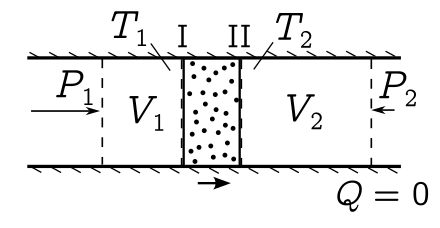
\includegraphics[width=0.7\textwidth]{1.png} % Имя файла без расширения
		\caption*{Приложение 1}
	\end{figure}
	\begin{figure}[h] % Окружение для подписи и выравнивания
		\centering
		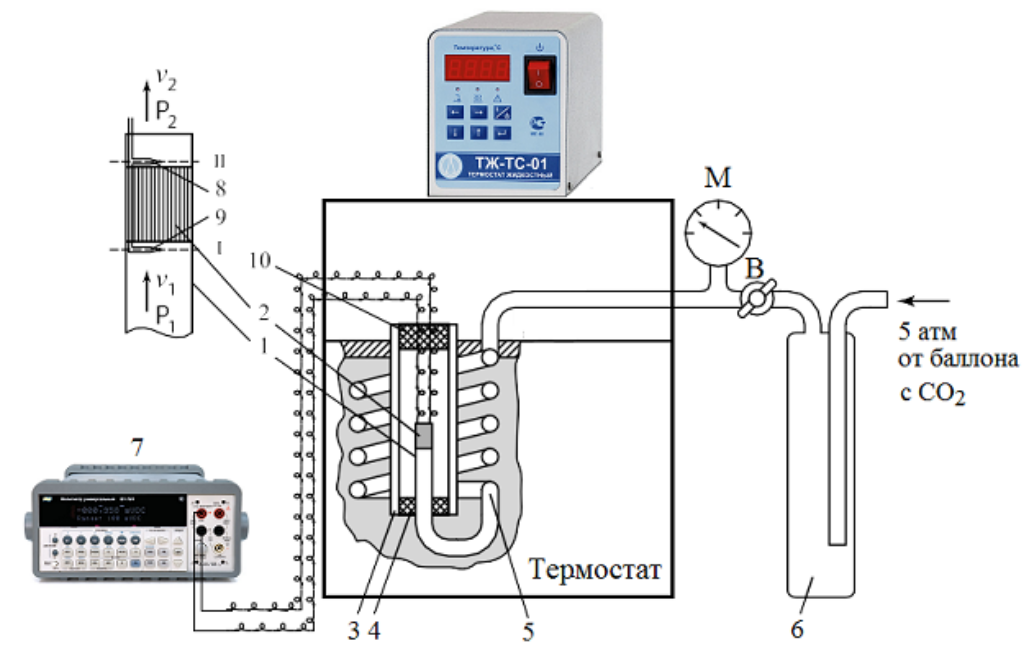
\includegraphics[width=1\textwidth]{2.png} % Имя файла без расширения
		\caption*{Приложение 2}
	\end{figure}
	\begin{figure}[h] % Окружение для подписи и выравнивания
		\centering
		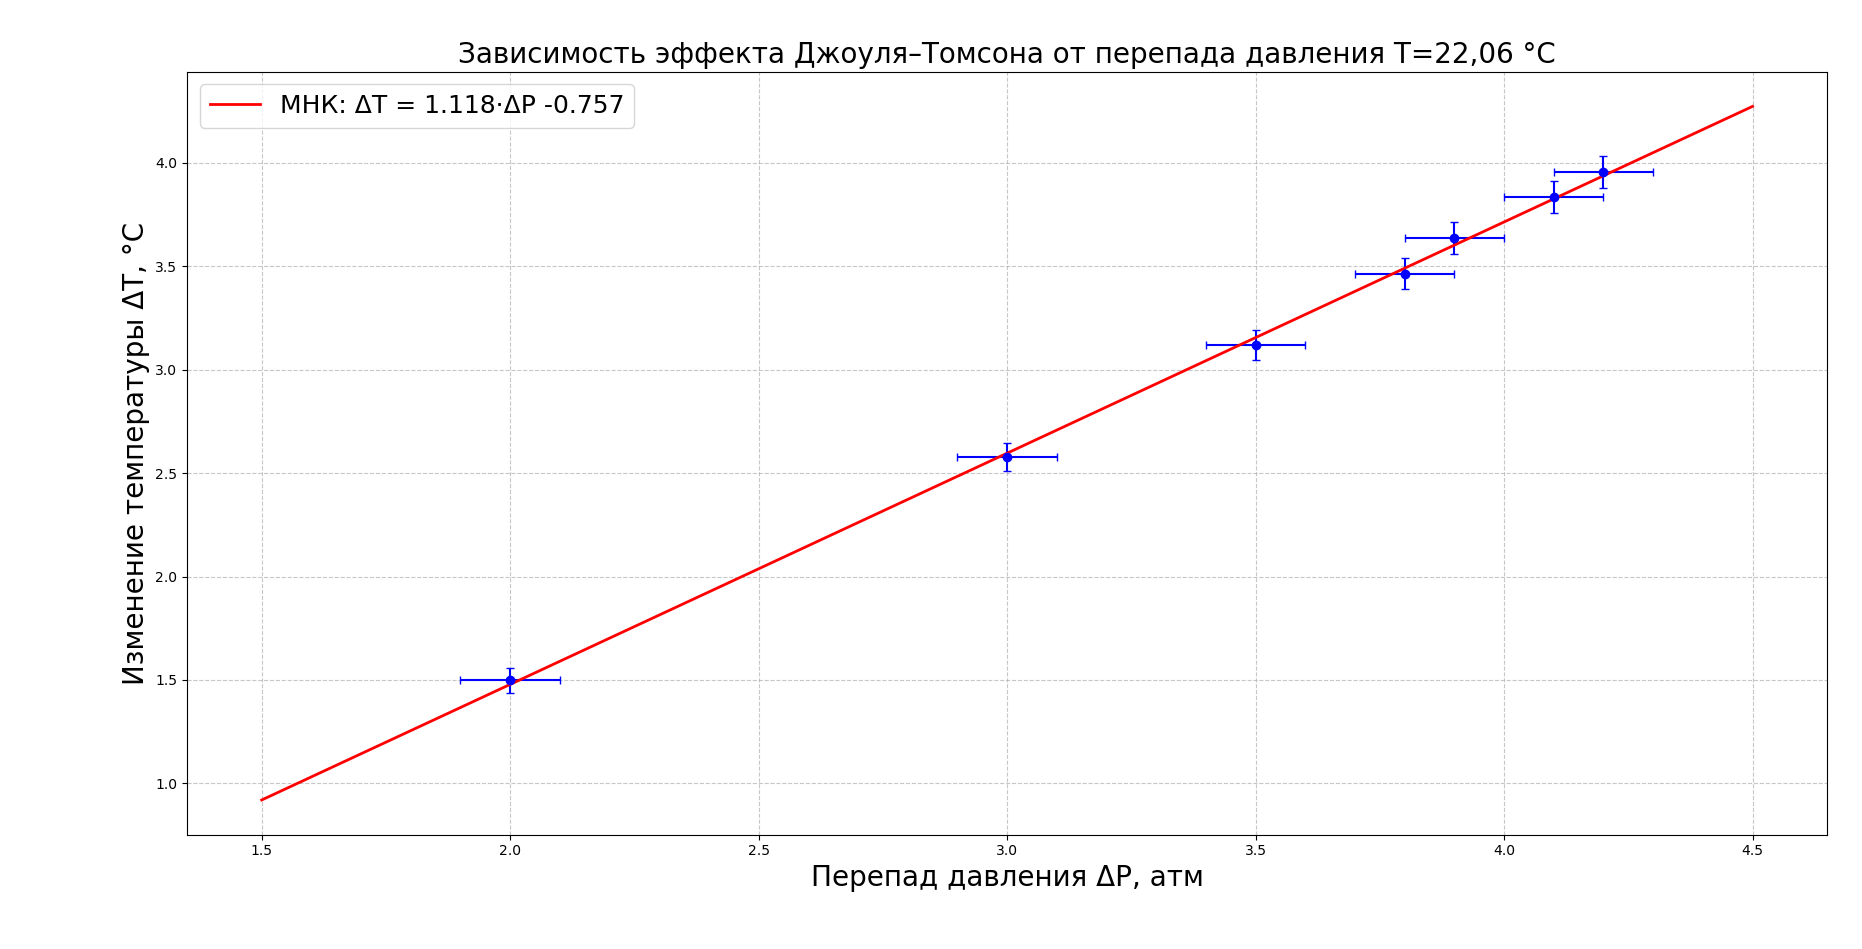
\includegraphics[width=1\textwidth]{20.png} % Имя файла без расширения
		\caption*{Приложение 3}
	\end{figure}
	\begin{figure}[h] % Окружение для подписи и выравнивания
		\centering
		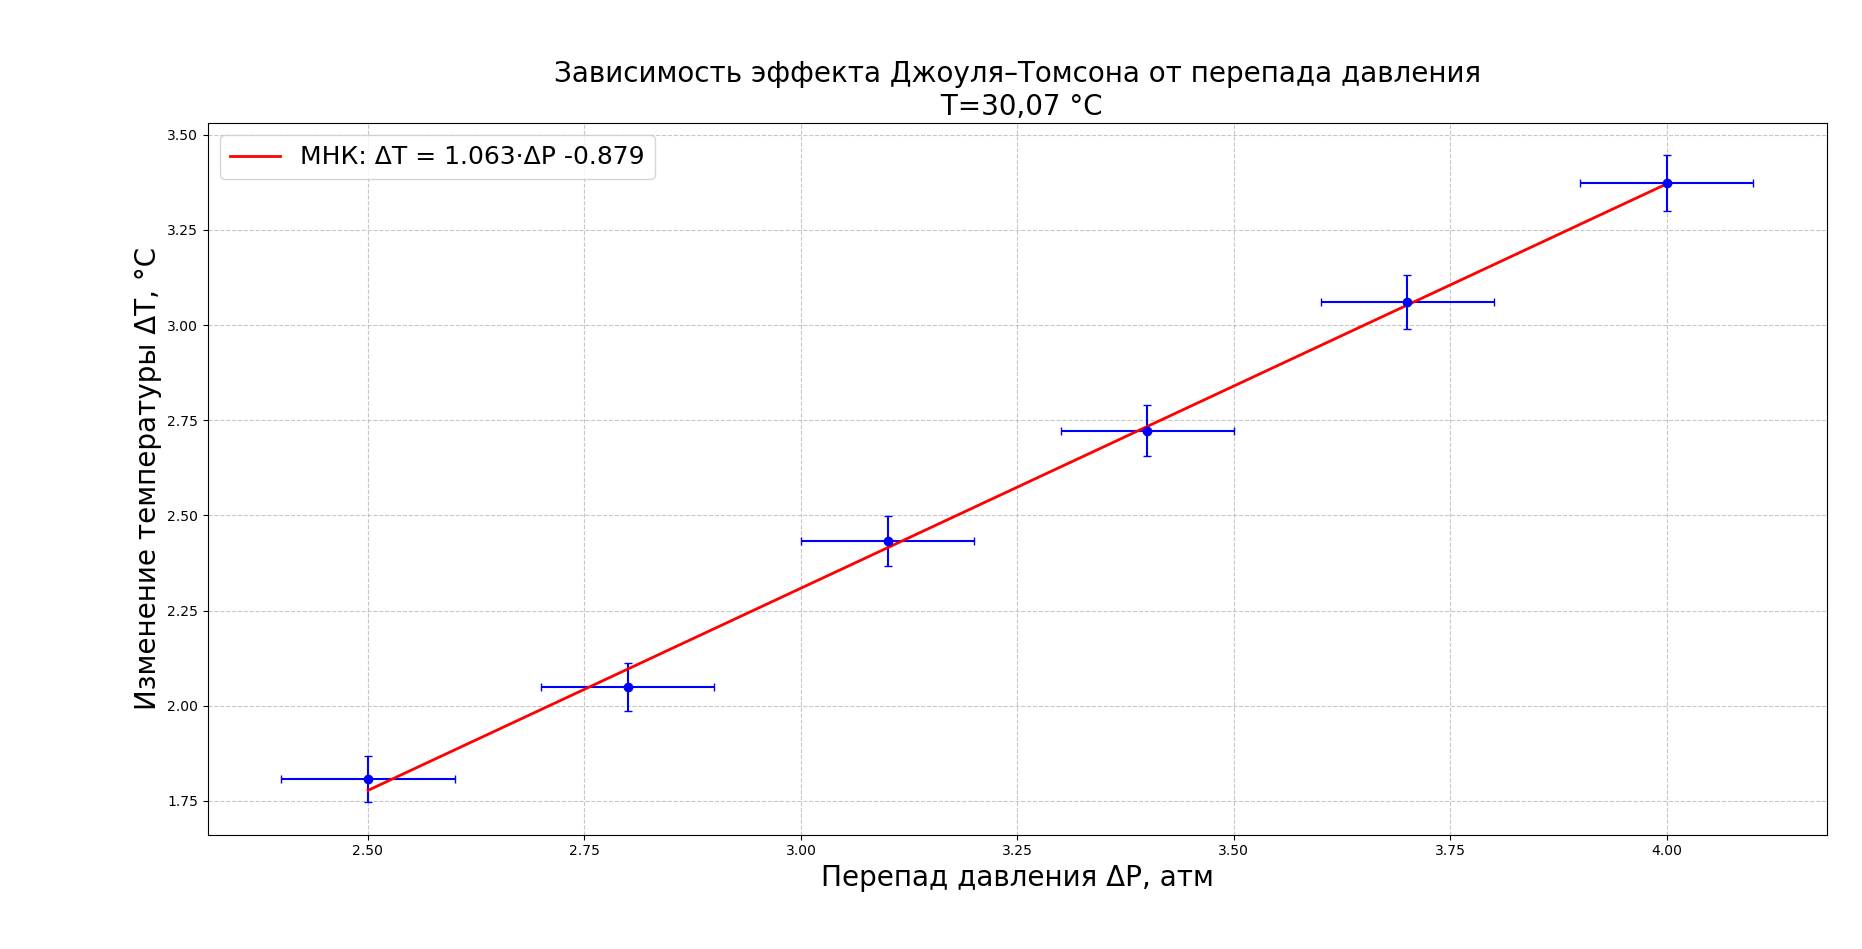
\includegraphics[width=1\textwidth]{30.png} % Имя файла без расширения
		\caption*{Приложение 4}
	\end{figure}
	\begin{figure}[h] % Окружение для подписи и выравнивания
		\centering
		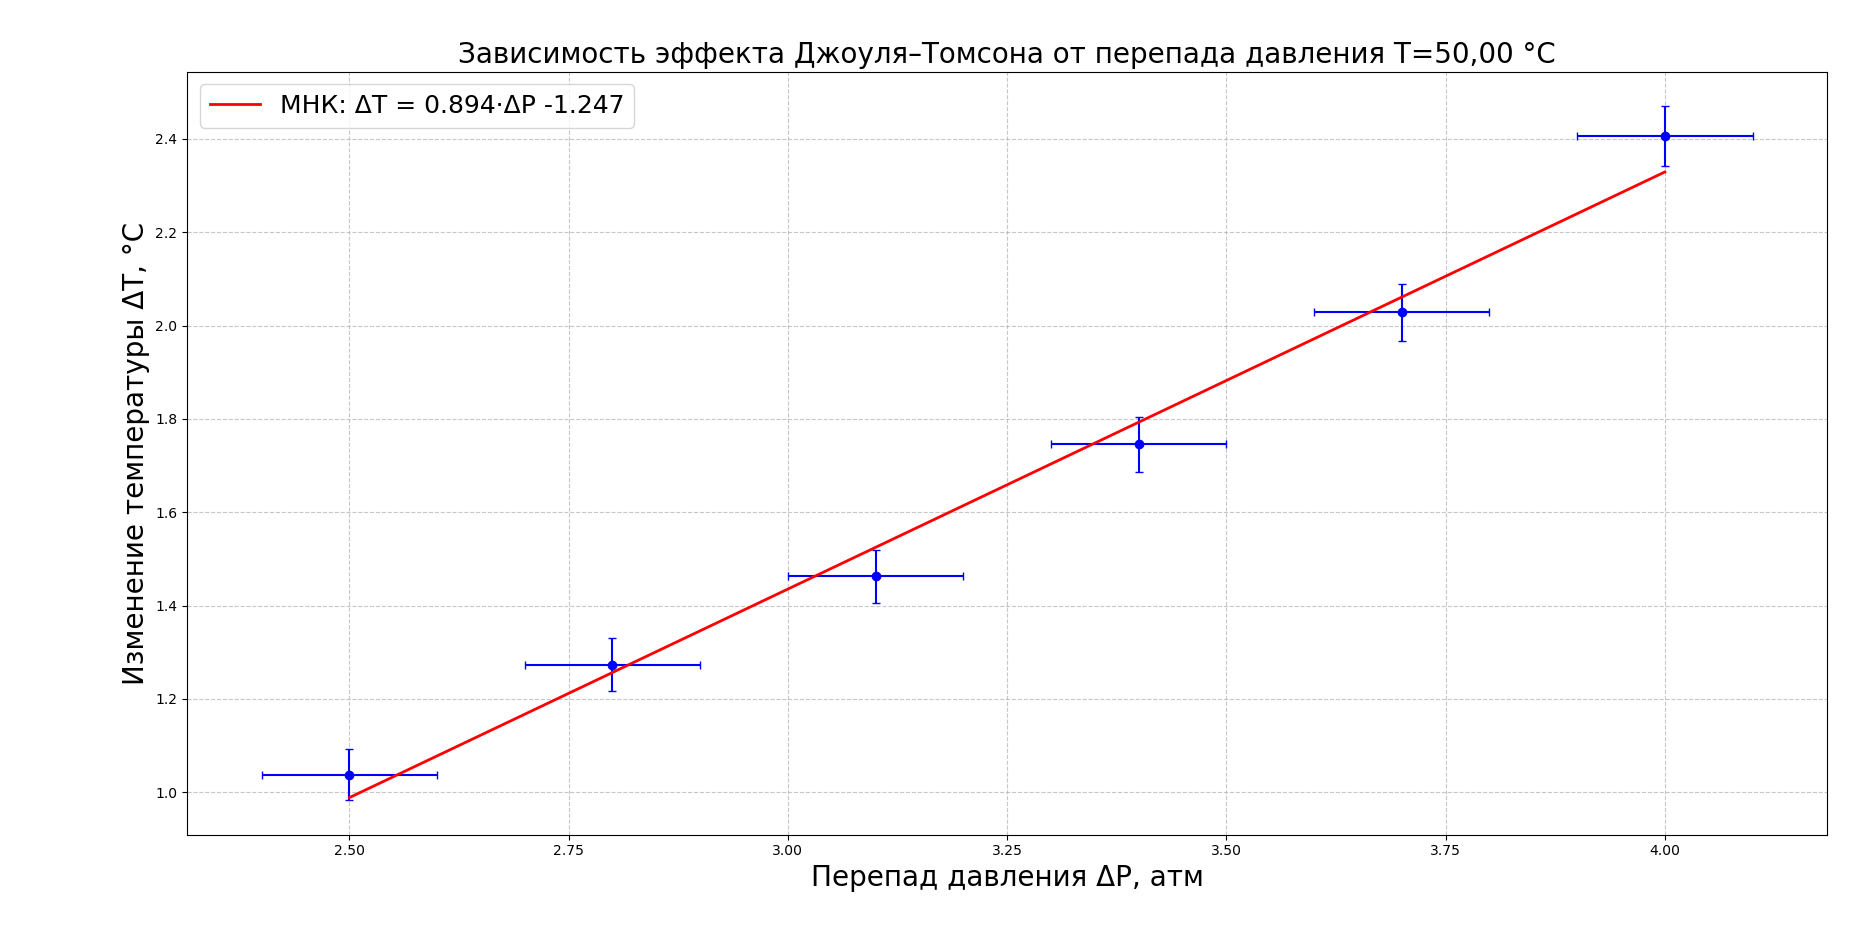
\includegraphics[width=1\textwidth]{50.png} % Имя файла без расширения
		\caption*{Приложение 5}
	\end{figure}
	\begin{figure}[h] % Окружение для подписи и выравнивания
		\centering
		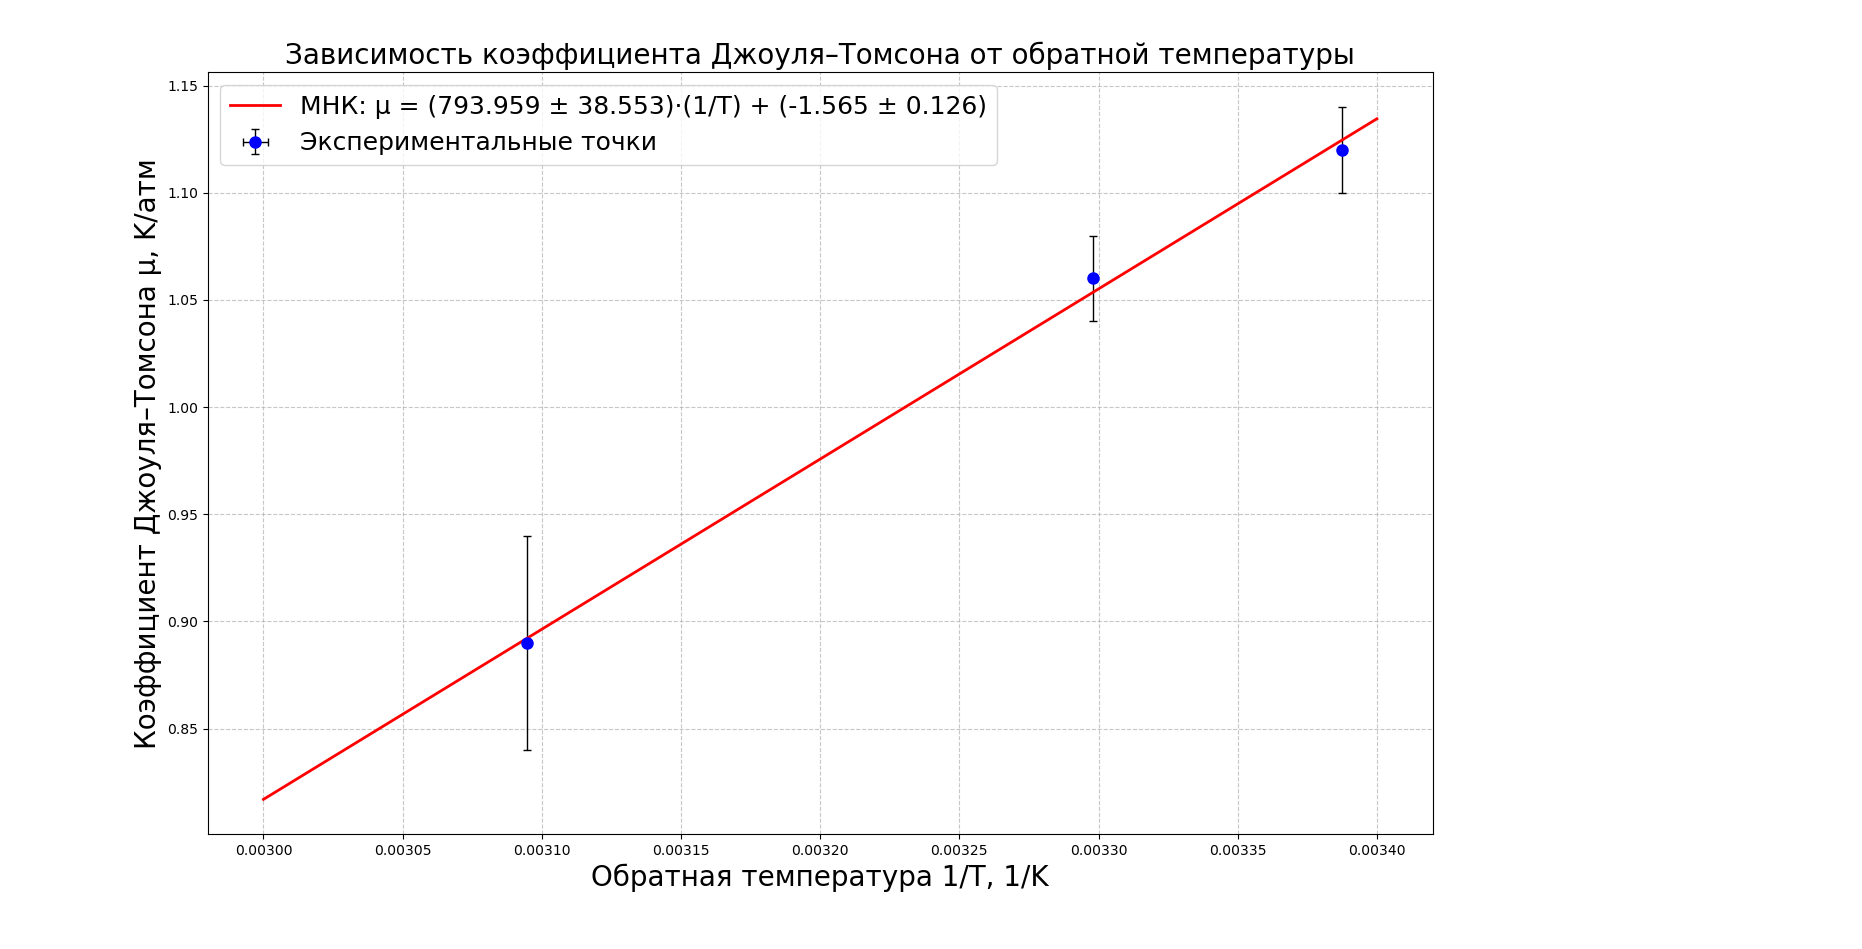
\includegraphics[width=1.2\textwidth]{kT.png} % Имя файла без расширения
		\caption*{Приложение 6}
	\end{figure}
\end{document}

